\section{Visioner om den samlede forandring}
\subsection{Teknologi}
%
% ! ER Diagram over de nye funktionalitere / visioner
%
\subsubsection{It-systemer og it-platform}
It-platformen for den samlede vision for MinSP er Sundhedsplatformen.
\\\\
\textbf{Prioritet 1, Receptfornyelse} \\
It-systemerne er udover MinSP også Sundhedsplatformen og muligvis apotekernes systemer og FMK (det fælles medicin kort), da der skal være integration i mellem disse systemer.
\\\\
\textbf{Prioritet 2, Samling af al information} \\
%
% ? - Anders Lassen: "Læring og videnscenter. Der er allerede patienthåndbogen Jeg tror det er out-of-scope":
%
Denne funktionalitet vil kunne løses med en 'standardløsning', da der allerede eksisterer flere troværdige informationssider, hvor det er læger, der vedligeholder siderne. \\
Viden og information om diabetes kan slås op i 'Patienthåndbogen'. Der findes allerede et link til 'Patienthåndbogen' i MinSP, men dette ligger 'gemt' i undermenuen 'Historik' under hovedmenuen 'Sundhedsdata'.
\\ \\
Under en menu 'Information om dine Diagnoser', kunne et link til 'Patienthåndbogen' placeres. \\
I samme menu kan der lægges et link til 'Diabetesforeningen', der tilbyder fællesskab mellem diabetikere i form af f.eks. motivationsgrupper og diabetescafér samt rådgivning til diabetikere.
\\
Endvidere kan et link til 'Steno Diabetes Center' give video-information omkring f.eks. 'Hvordan man måler blodglukose', en diætist der fortæller om 'Kulhydrattælling' og informerer om kost og motion. og en overlæge der fortæller om 'Graviditetsdiabetes' m.fl. \\
På siden er der også information om blandt andet det at være ny med diabetes, til gravide med diabetes, hjælp til at forstå tal, madopskrifter og meget meget mere. 
\\ \\
Disse 'standardløsninger' kan være en måde til at løse funktionaliteten 'Samling af al information', og dermed undgås en dyr løsning, hvor hospitalernes sundhedspersonale skal vedligeholde egen udviklede informationssider på MinSP.
\\\\
\textbf{Prioritet 3, Uniforme Prøvesvar} \\
It-systemerne er udover MinSP også Sundhedsplatformen og FMK, da der skal være integration i mellem disse systemer.
\subsubsection{Funktion}  
% ? - Indenholde: 'Liste over de enkle it-systemers funktioner'
\textbf{Prioritet 1, Receptfornyelse}\\
Receptfornyelse er en funktionalitet (/vision - ?), der skal ny-udvikles. Kravet til funktionaliteten skal være, så patienter, i MinSP, selv kan aktivere fornyelse af en eller flere recepter for deres ordinerede medicin. 
\\
Receptfornyelsen skal være synlig og skal derfor placeres som en hovedmenu øverst på MinSP. Undermenuen til hovedmenuen 'Receptfornyelse' skal indeholde: 'Forny recept', 'Medicin kort' og 'Historik'.
\\
Man skal kunne følge gangen i receptfornyelsen fra status 'Medicin bestilt' til 'Medicin kan hentes på apoteket'. Man skal også kunne vælge modtager-apotek, med to valgmuligheder, samt om man ønsker en påmindelse om receptfornyelse og i hvilken form (sms, besked i app'en, privat mail eller eboks). 
\\ 
Recept skal kun kunne fornys, når sidst udleverede dosis er ved slippe op.  
\\
'Medicinkortet' skal indeholde en liste over ordineret medicin.\\ 
'Historik' skal indeholde en liste over alle udleveringer af medicin til dato.
\\ \\
Vi vurderer, at 'Receptfornyelse' er en kompliceret funktionalitet, da den skal ny-udvikles, og da der er ikke noget eksisterende funktionalitet, der kan genbruges. Funktionaliteten er også kompliceret, fordi sikkerheden skal være høj i forhold til, at der ikke må udleveres for meget medicin, og da det kun er den ordinerede medicin, der må fornys. \\
Udviklingen af statuslinje, for gangen i receptfornyelsen, vil også være kompliceret, fordi registreringen skal overføres af sundhedspersonalet fra Sundhedsplatformen til MinSP.\\
Modtagerapotek skal kunne vælges i forhold til bopæl, og det vurdere vi også vil være kompliceret, fordi der skal bruges data omkring hvor alle apoteker i Region Sjælland ligger.\\
Påmindelse vil kræve, at der beregnes en dato for fornyelse af recept i forhold til tid eller dosis ved sidste fornyelse. Dette vurderes igen at være kompliceret at udvikle, fordi der skal være en database hvor oplysninger om ordineret medicin, historikken for udleveret medicin og receptfornyelser gemmes. \textcolor{red}{(findes den eller skal den udvikles - ?)} \\ 
Til patient databasen skal der tilknyttes attributterne 'Primær apotek' og 'Sekundær apotek'.
\\\\
\textbf{Prioritet 2, Samling af al information} \\
Et forslag til at imødekomme visionen om en 'Samling af al information' kunne være, at tilføje under hovedmenuen Profil, at tilføje en undermenu 'Information om dine diagnoser'. Under denne undermenu kan der placeres link til f.eks. Patienthåndbogen, Diabetesforeningen og Steno Diabetes Center.
\\\\ 
\textbf{Prioritet 3, Uniforme Prøvesvar} \\
Denne funktionalitet vil kunne løses ved, at man til hvert enkelt prøvesvar knytter en forklaring af prøve-typen på dansk. Der skal her udover angives, hvor prøven er taget (hospital, læge, laboratorie).\\
Prøvesvarene skal holdes adskilt pr. diagnoses, hvis patienten har flere diagnoser.\\
Eksisterende database / tabel med prøvesvar skal have tilknyttet en attribut med forklarende tekst på dansk, om hvad prøven viser, og en attribut med navn på hospital / læge / laboratorie. Derfor skal der være en tabel med hospitals- / læge- / laboratorie navne, som navnet kan hentes fra.\\ 
Tekstbeskrivelsen kan være en standard tekst pr. prøvetype, men navet på stedet, hvor prøven er taget, kan variere. Dette skal derfor indrapporteres af personalet, når prøvesvar indrapporteres. \\
At holde prøvesvar adskilt pr. diagnose kræver, at der i prøvesvar tabellen skal være en attribut for diagnose, som så for hvert prøvesvar skal udfyldes med relevant diagnose af sundhedspersonalet.\\
\subsubsection{Brugergrænseflader} % Krav til Brugergrænseflader
Brugergrænsefladerne skal designes så de overholder GUI-guidelines for god interaktions design. %  Benyon s. 88 
\\\\
\textbf{Prioritet 1, Receptfornyelse} \\
Implementering af receptfornyelses funktionaliteten vil kræve integration med Sundhedsplatformens medicinmodul og apotekerenes systemer. 
Der skal være en ny grænseflade mellem MinSP og FMK.\\\\
Forslag til brugergrænseflade for patienten fremgår af nedenstående Mock-up's:\\
\begin{figure}[H]
	\centering
	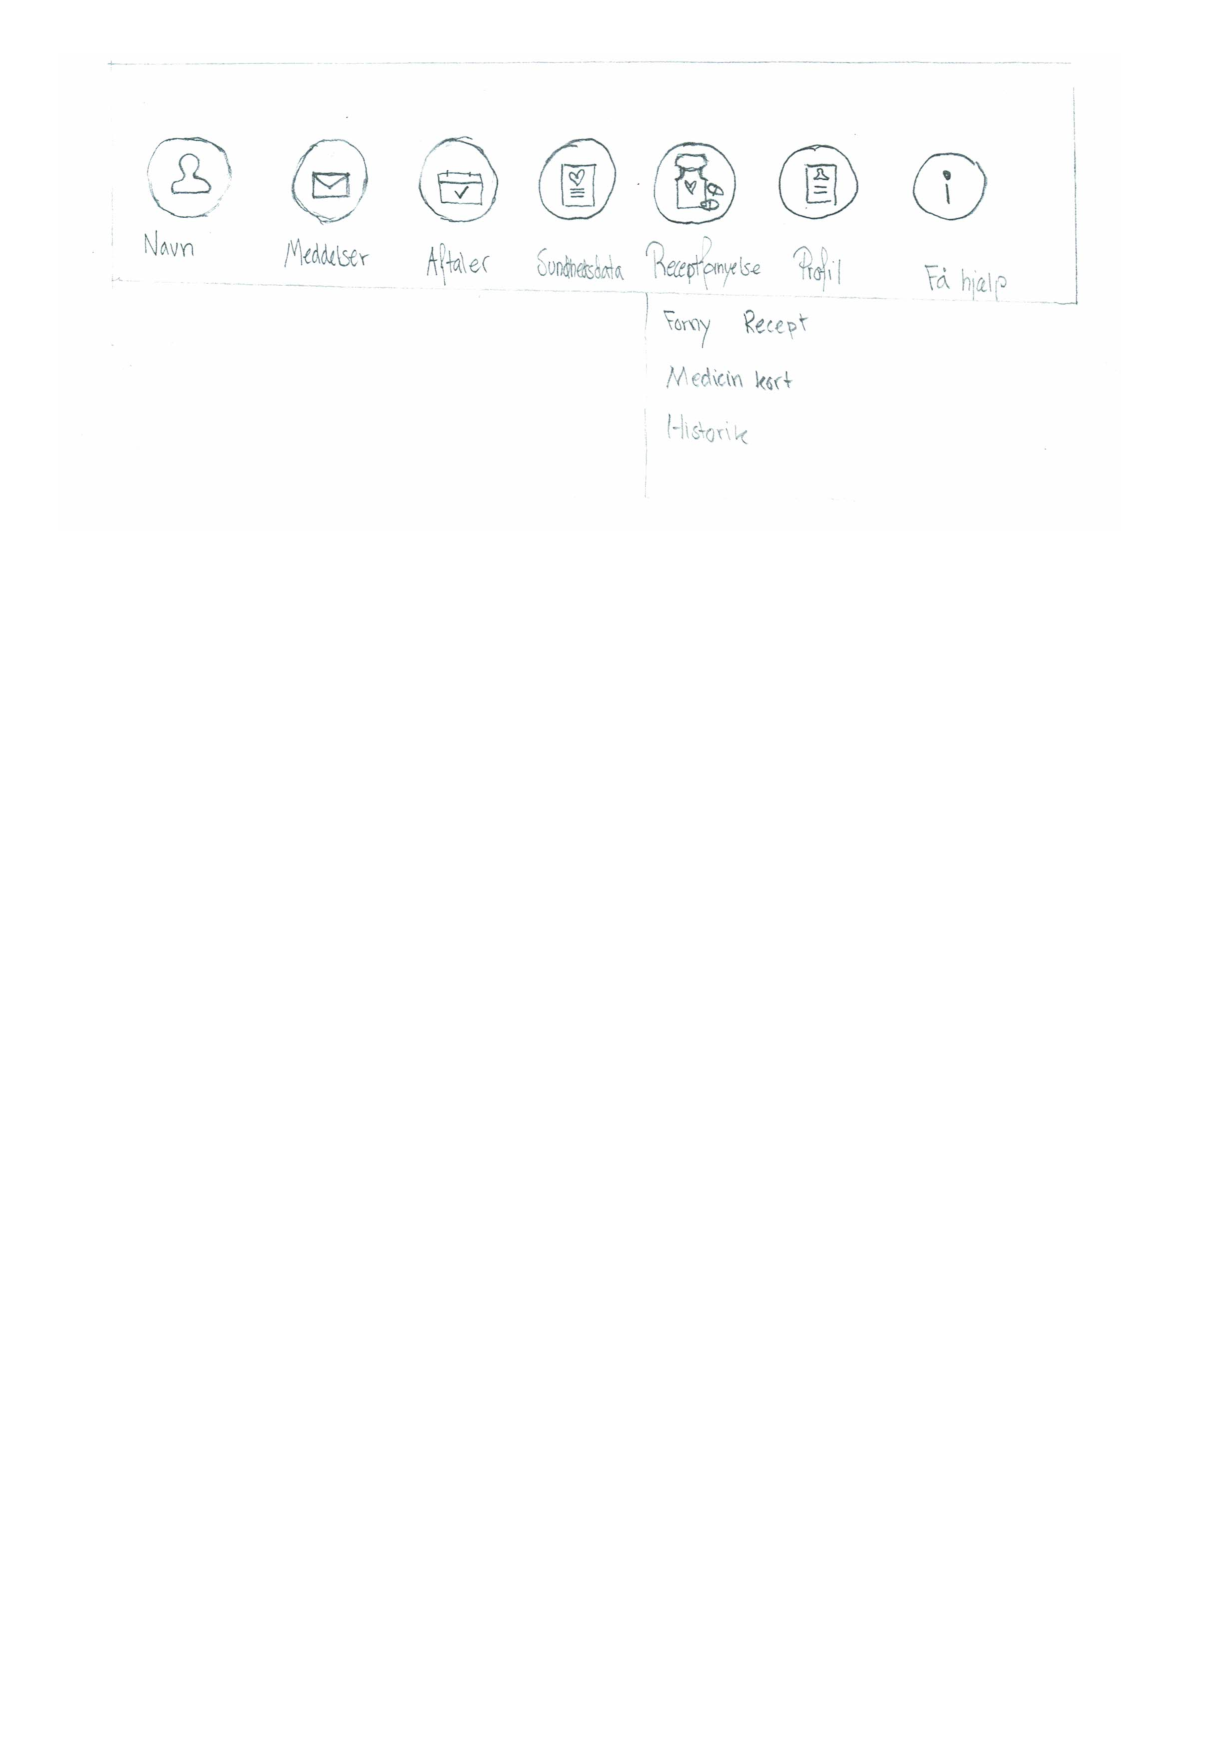
\includegraphics[angle=0, height=0.36\textheight]{Materials/FornyRecept_Hovedmenu.pdf}
	\caption{Mock-up for modulet 'Receptfornyelse': Hovedmenuen}
	\label{fig:Mock-Up}
\end{figure}
\begin{figure}[H]
	\centering
	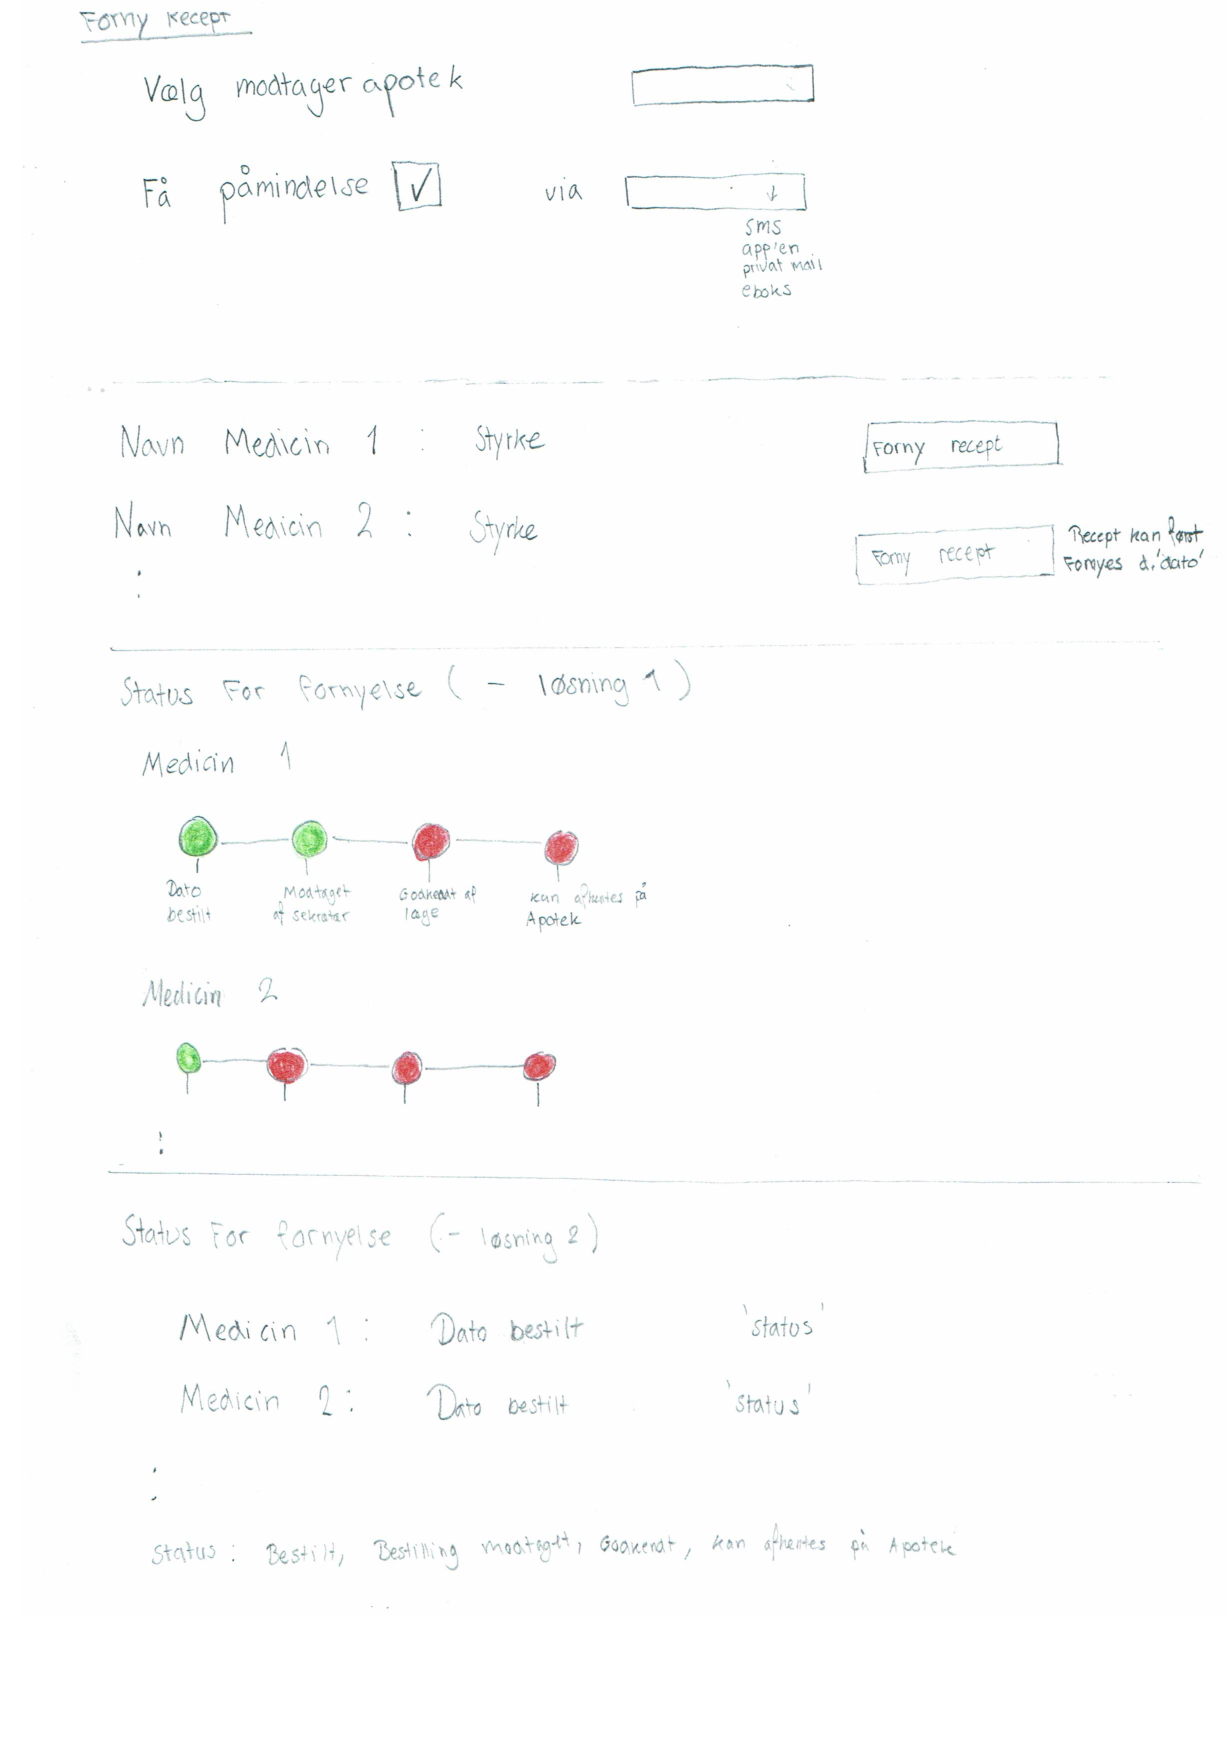
\includegraphics[angle=0, height=0.85\textheight]{Materials/FornyRecept.pdf}
	\caption{Mock-up for modulet 'Receptfornyelse': Undermenu, 'Forny recept'}
	\label{fig:Mock-Up}
\end{figure}
\begin{figure}[H]
	\centering
	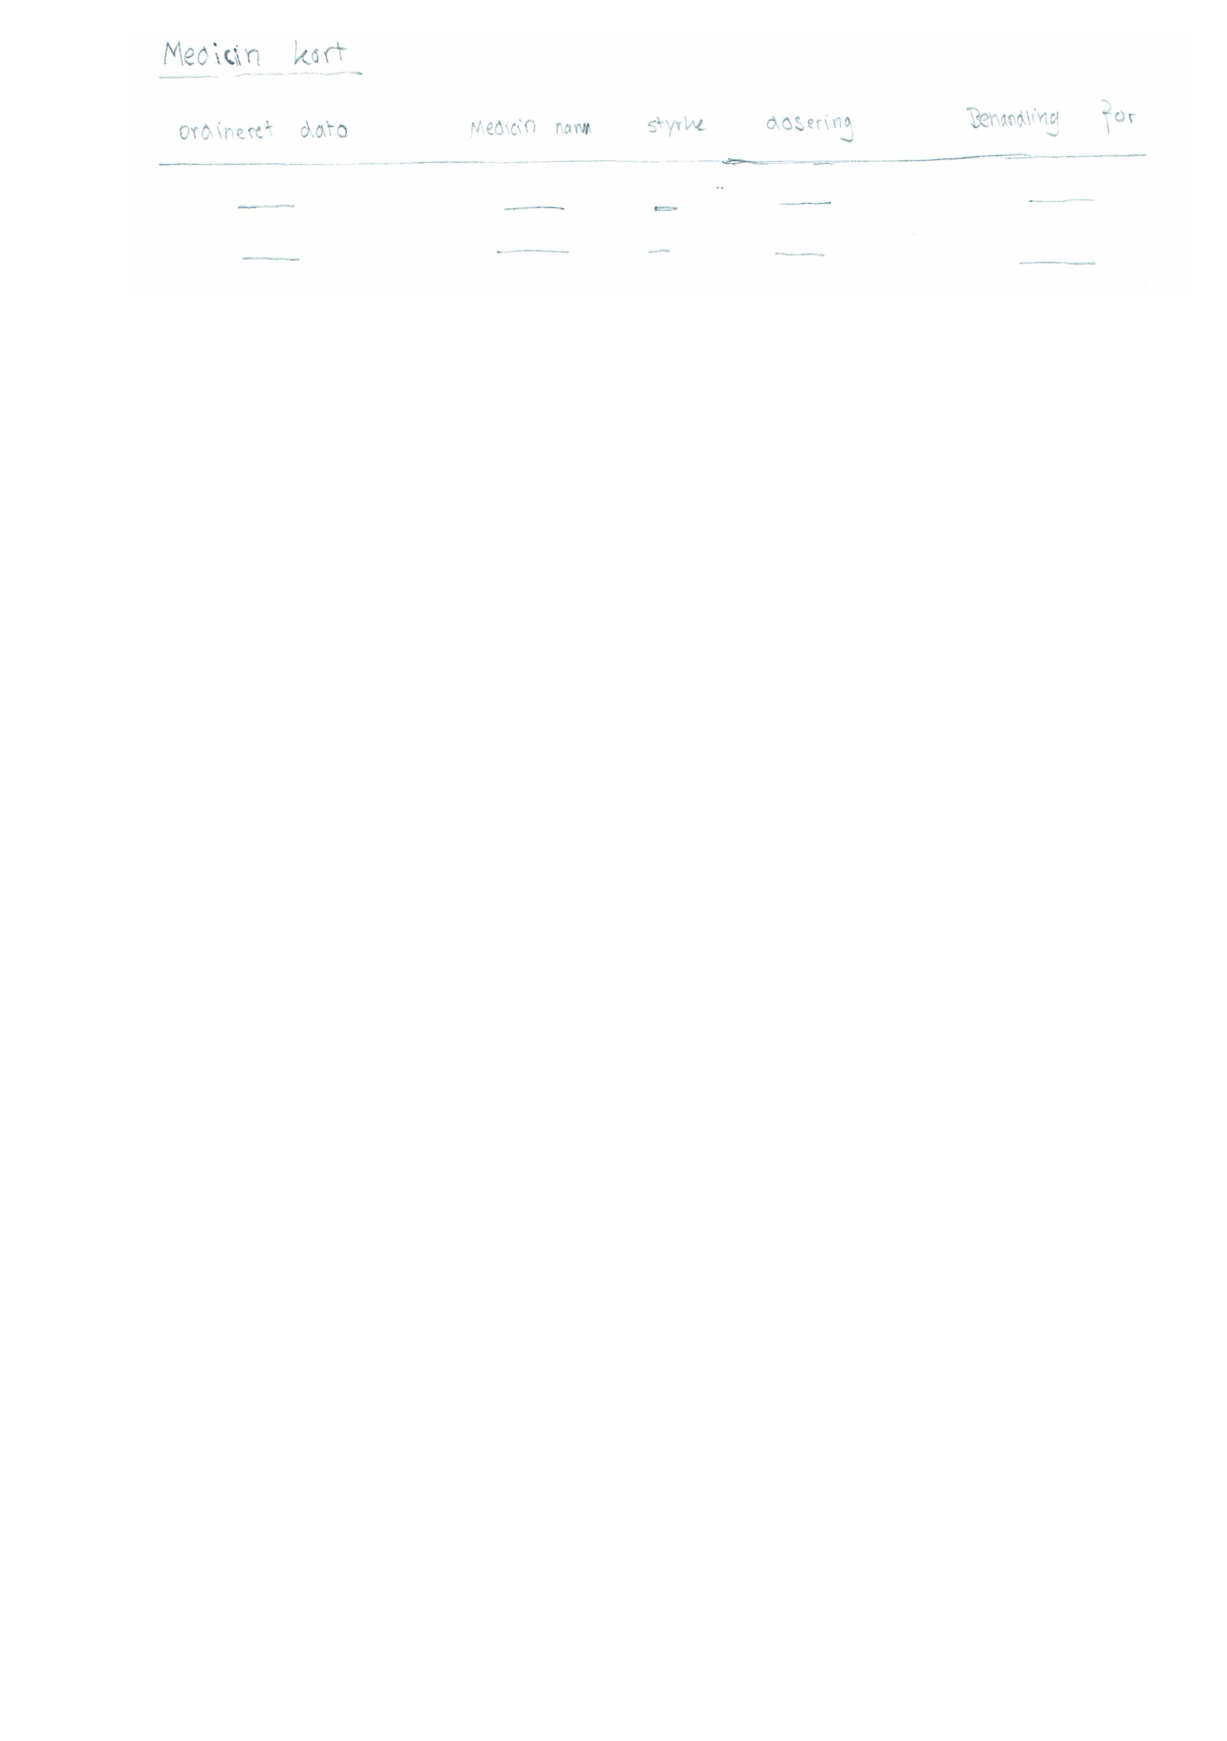
\includegraphics[angle=0, height=0.2\textheight]{Materials/FornyRecept_Medicinkort.pdf}
	\caption{Mock-up for modulet 'Receptfornyelse': Undermenu, 'Medicin kort'}
	\label{fig:Mock-Up}
\end{figure}
\begin{figure}[H]
	\centering
	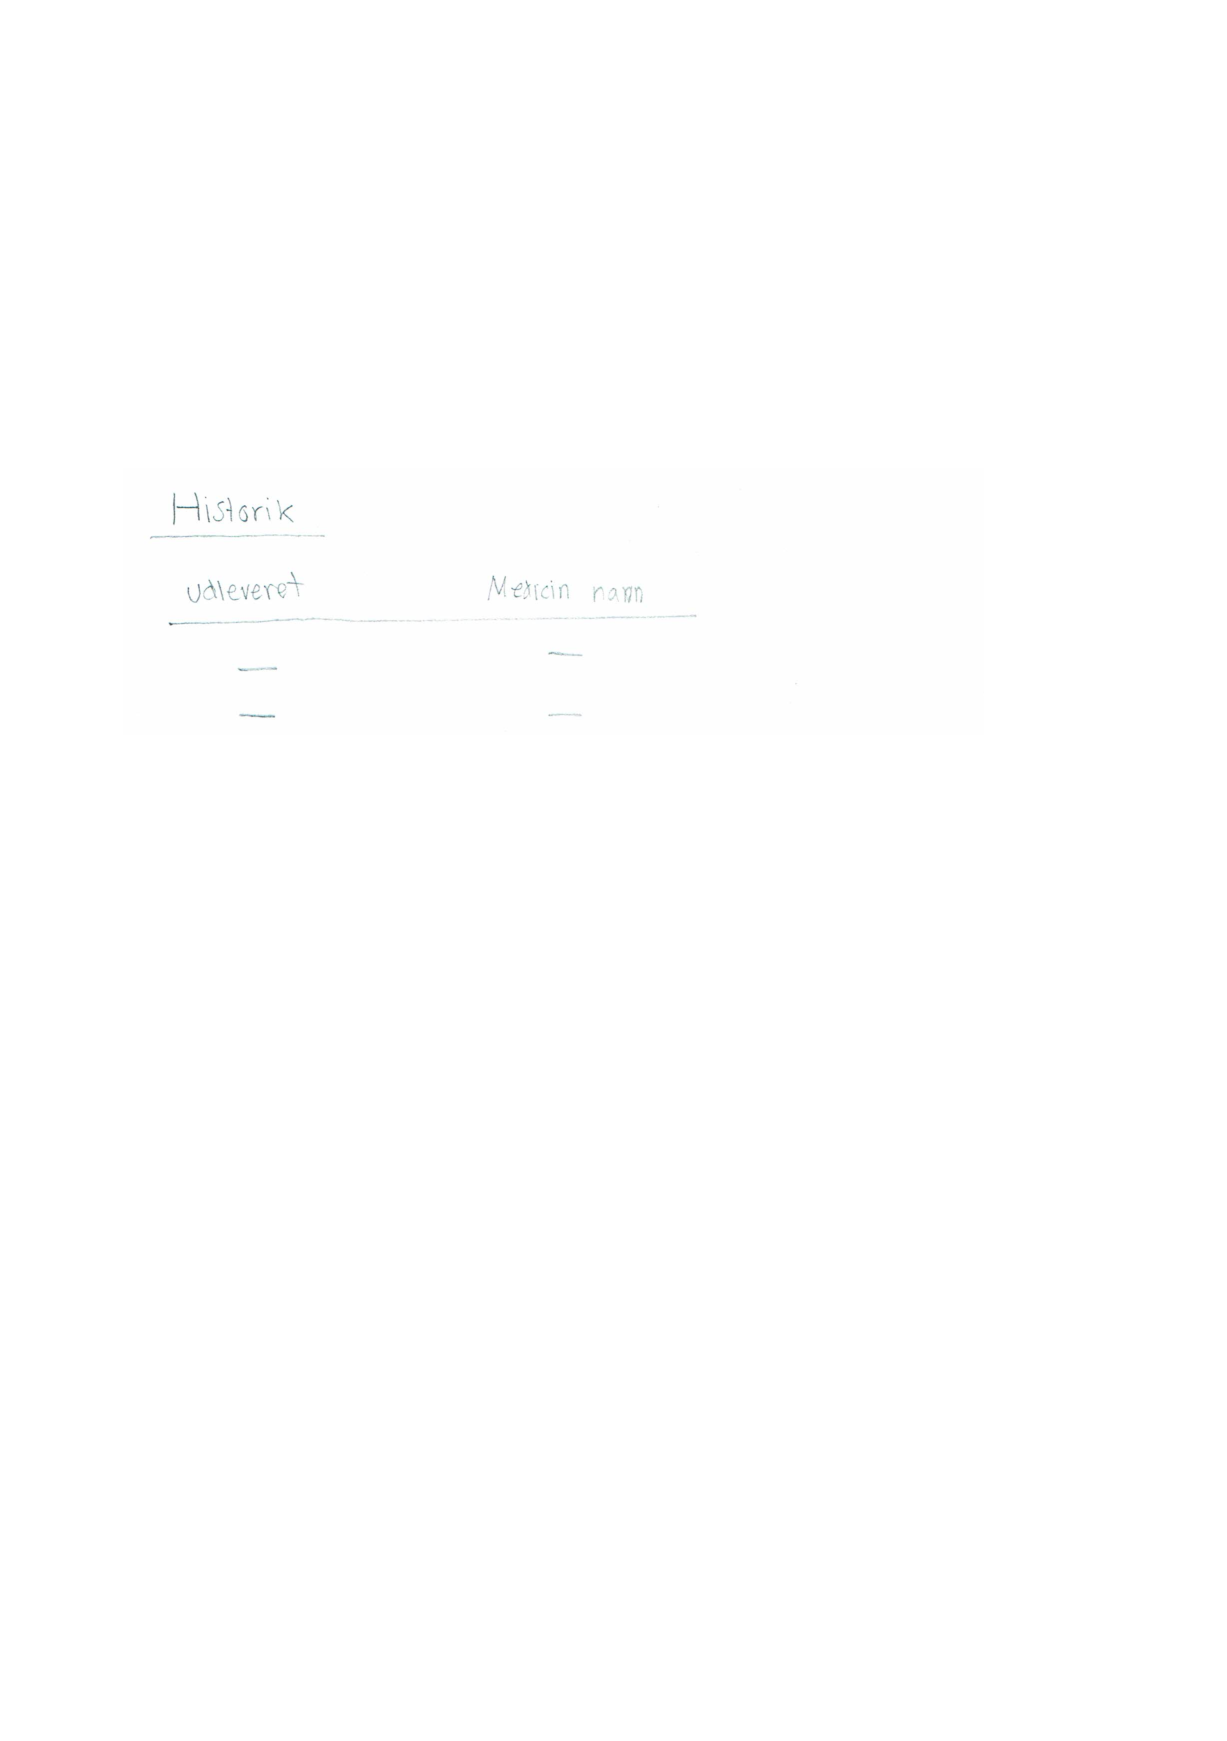
\includegraphics[angle=0, height=0.2\textheight]{Materials/FornyRecept_Historik.pdf}
	\caption{Mock-up for modulet 'Receptfornyelse': Undermenu, 'Historik'}
	\label{fig:Mock-Up}
\end{figure}
% ? - Scenarios
\textbf{Prioritet 2, Samling af al information} \\
Forslag til brugergrænseflade for patienten fremgår af nedenstående Mock-up's:\\
\begin{figure}[H]
	\centering
	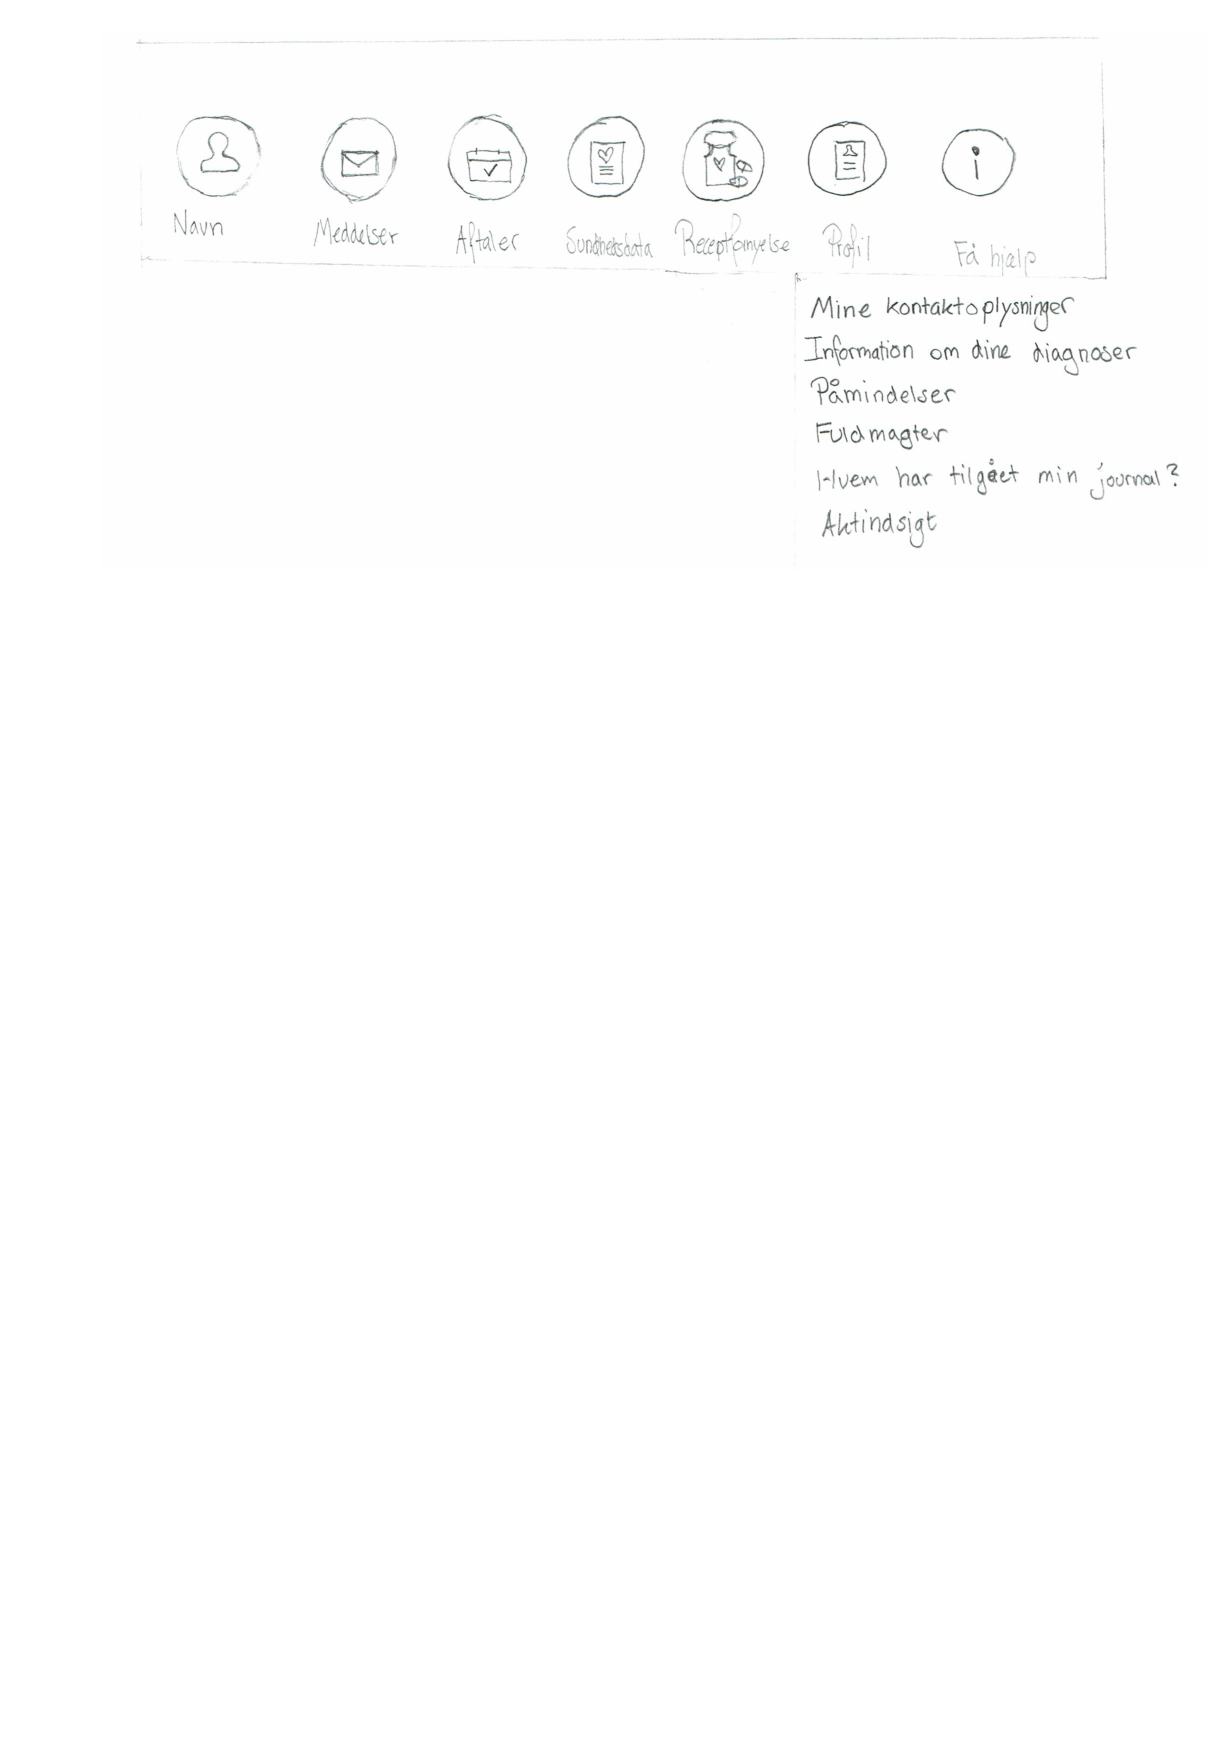
\includegraphics[angle=0, height=0.3\textheight]{Materials/Information_Hovedmenu.pdf}
	\caption{Mock-up for modulet 'Information om dine diagnoser': Hovedmenu, 'Profil'}
	\label{fig:Mock-Up}
\end{figure}
\begin{figure}[H]
	\centering
	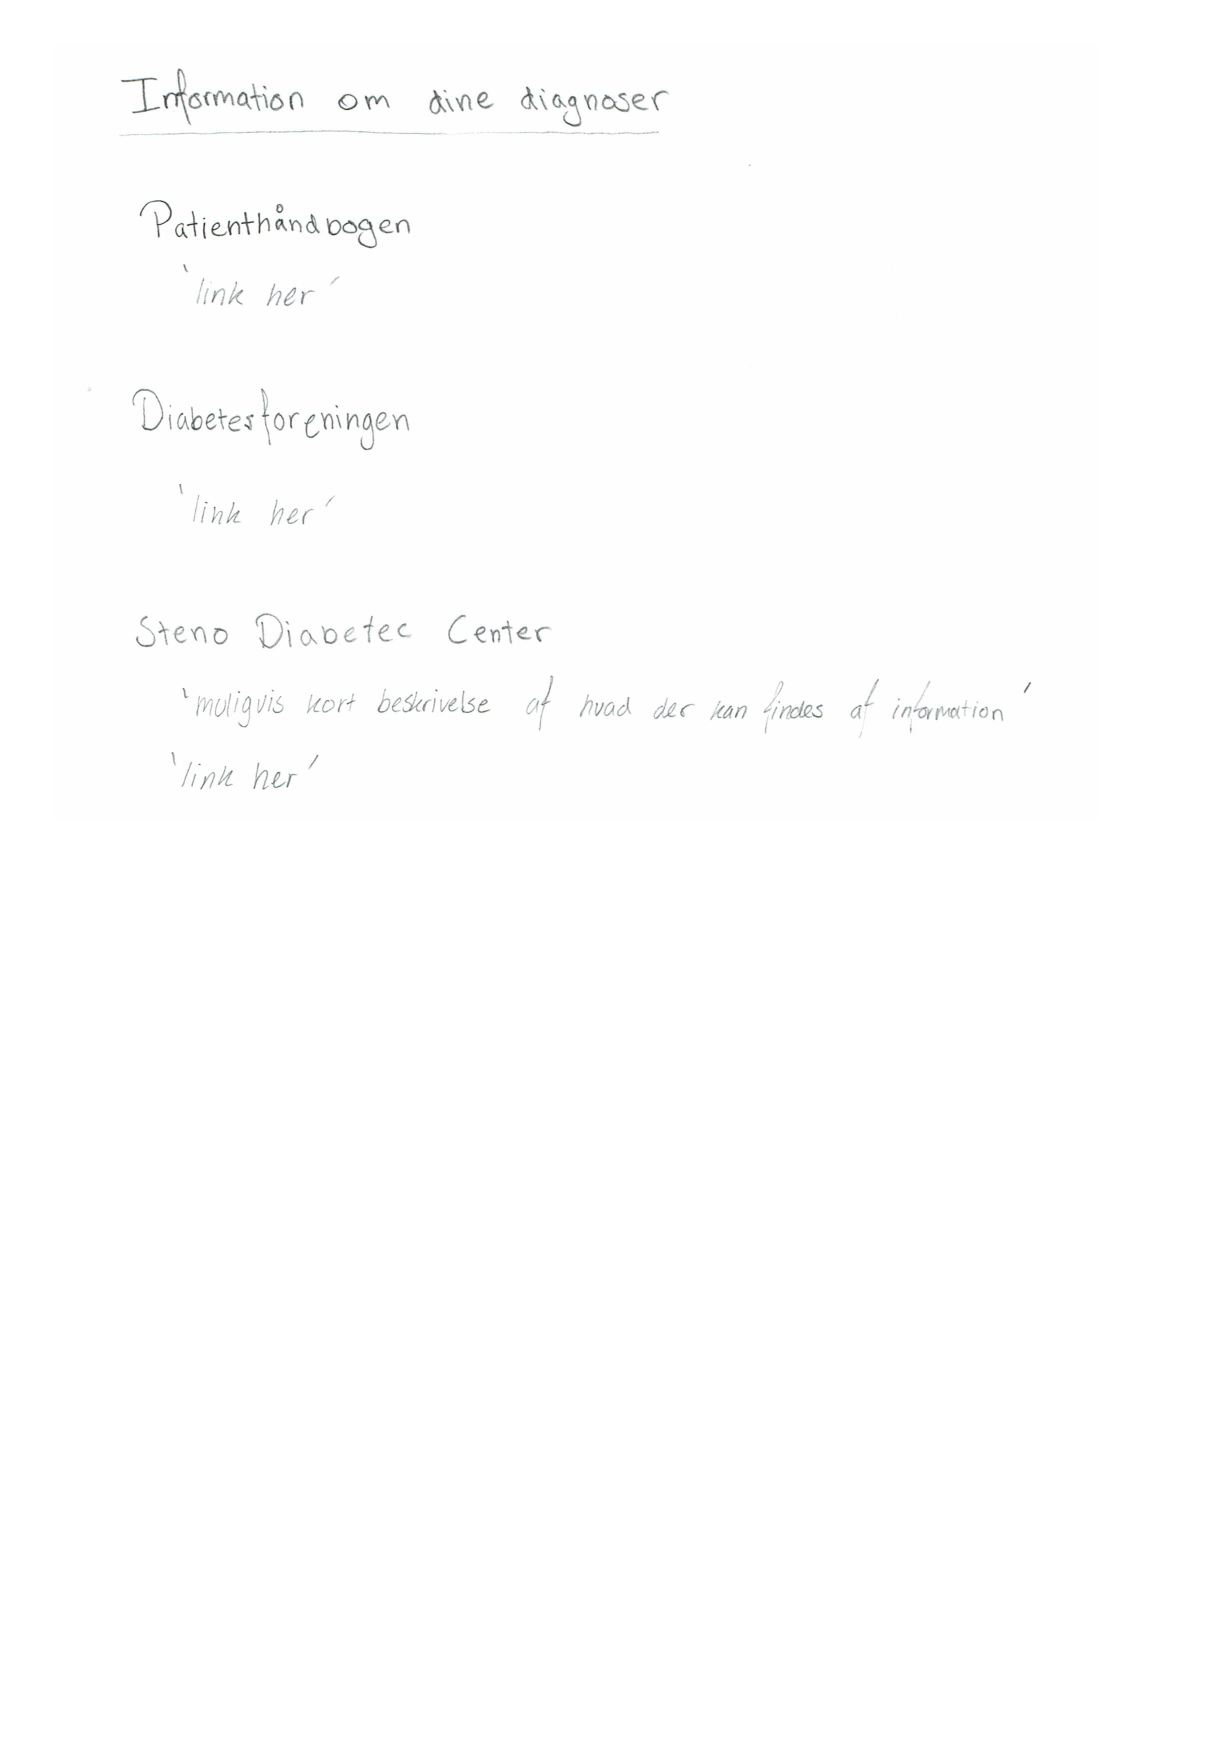
\includegraphics[angle=0, height=0.44\textheight]{Materials/Information.pdf}
	\caption{Mock-up for modulet 'Information om dine diagnoser': Undermenu}
	\label{fig:Mock-Up}
\end{figure}
\textbf{Prioritet 3, Uniforme Prøvesvar} \\
Forslag til brugergrænseflade for patienten fremgår af nedenstående Mock-up's:\\
\begin{figure}[H]
	\centering
	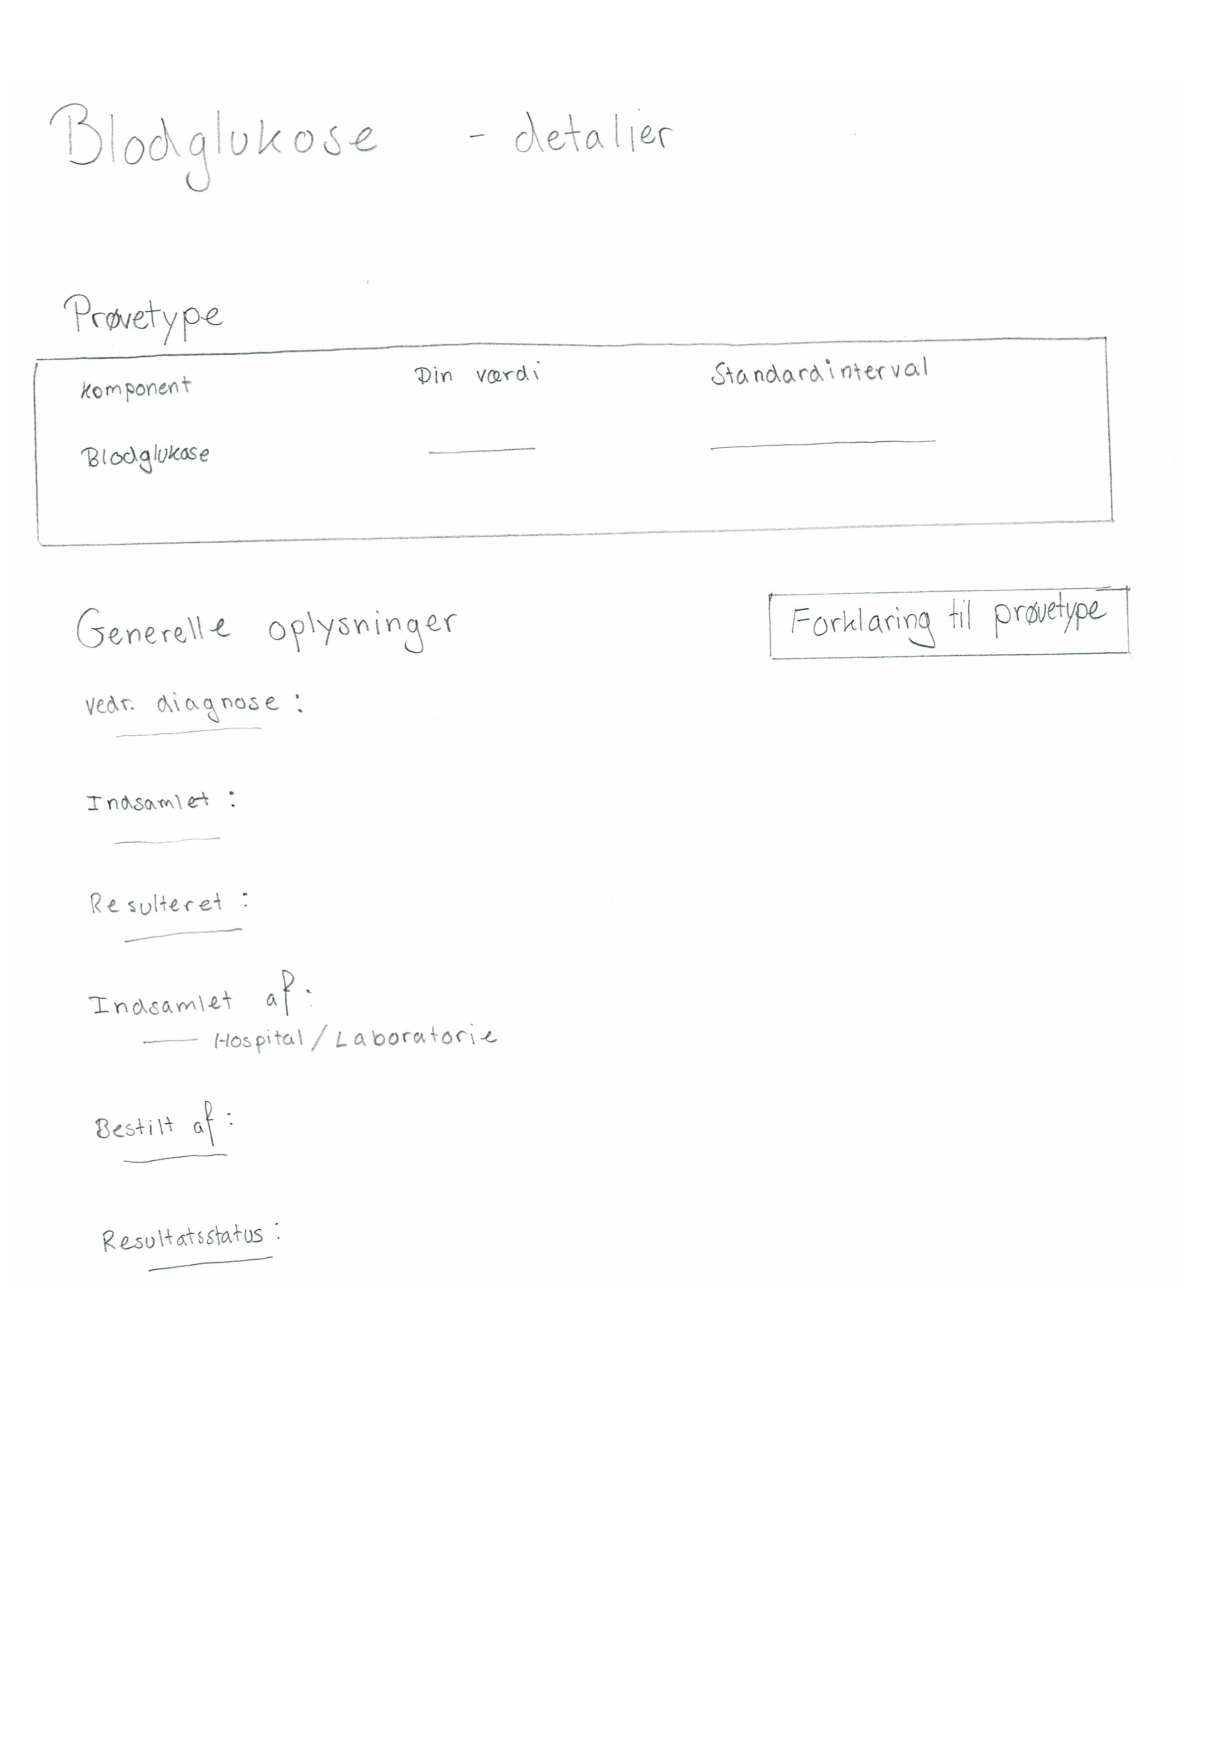
\includegraphics[angle=0, height=0.7\textheight]{Materials/provesvar.pdf}
	\caption{Mock-up for modulet 'Prøvesvar'}
	\label{fig:Mock-Up}
\end{figure}

\subsection{Arbejdets organisering}  
\textbf{Prioritet 1, Receptfornyelse} \\
En automatisk receptfornyelse vil muligvis ændre arbejdsgangen for sundhedspersonalet. \\ 
Vi tænker at lægen fortsat stadigvæk skal tjekke, at ordineringen er korrekt i forhold til journalen, men at læge-sekretæren slipper for at skrive besked tilbage til patienten, da patienten nu selv kan se forløbet i statuslinjen.
%
\textcolor{red}{ - evt. udarbejde et scenarie for arbejdsgangen for sundhedspersonalet i forhold til Receptfornyelse.}
\\\\
\textbf{Prioritet 2, Samling af al information} \\
Hvis funktionaliteten implementeres via links, som forslået, vil der ikke være nogen ændringer til arbejdsgange og arbejdets organisering. \\
Hvis ikke funktionaliteten implementeres via links, men som en ny-udviklet informationside, er det sundhedspersonalet der skal skrive alt informationen / optage videoer mv og siden vil skulle vedligeholdes af sundhedspersonalet, så det ville være en ekstra opgave, som sundhedspersonalet (læger, diætister og sygeplejeskær m.fl.) herved bliver pålagt.
\\\\
\textbf{Prioritet 3, Uniforme Prøvesvar} \\
Funktionaliteten vil give ekstra arbejde for lægesekretærer eller laboratorie medarbejdere i forhold til indrapporteringen af prøvesvar, da der vil flere informationer, der skal indtastes. Der vil forinden være ekstra arbejde for lægen, da det er denne, der skal informere laboratorie-personale eller lægesekretær om hvilken diagnose de enkle prøvesvar vedrøre.\\
Der skal tages stilling til hvor i organisationen indrapporingen skal fortages.
\subsection{Kvalifikationsbehov}
\textbf{Prioritet 1, Receptfornyelse} \\
Receptfornyelses funktionaliteten vil ikke kræve nogen større oplæring af sundhedspersonalet, kun en introduktion til hvordan den nye funktionalitet fungerer.
\\\\
\textbf{Prioritet 2, Samling af al information} \\
Hvis funktionaliteten implementeres via links, vil det ikke kræve nogen oplæring af sundhedspersonalet.
\\\\
\textbf{Prioritet 3, Uniforme Prøvesvar} \\
Vores vurdering er, at ændringerne ikke kræver ekstra kvalifikationer.